% Copyright 2016 - 2018 Bas van Meerten and Wouter Franssen
%
%This file is part of Jellyfish.
%
%Jellyfish is free software: you can redistribute it and/or modify
%it under the terms of the GNU General Public License as published by
%the Free Software Foundation, either version 3 of the License, or
%(at your option) any later version.
%
%Jellyfish is distributed in the hope that it will be useful,
%but WITHOUT ANY WARRANTY; without even the implied warranty of
%MERCHANTABILITY or FITNESS FOR A PARTICULAR PURPOSE.  See the
%GNU General Public License for more details.
%
%You should have received a copy of the GNU General Public License
%along with Jellyfish. If not, see <http://www.gnu.org/licenses/>.

\documentclass[11pt,a4paper]{article}
% Copyright 2016 - 2018 Bas van Meerten and Wouter Franssen
%
%This file is part of ssNake.
%
%ssNake is free software: you can redistribute it and/or modify
%it under the terms of the GNU General Public License as published by
%the Free Software Foundation, either version 3 of the License, or
%(at your option) any later version.
%
%ssNake is distributed in the hope that it will be useful,
%but WITHOUT ANY WARRANTY; without even the implied warranty of
%MERCHANTABILITY or FITNESS FOR A PARTICULAR PURPOSE.  See the
%GNU General Public License for more details.
%
%You should have received a copy of the GNU General Public License
%along with ssNake. If not, see <http://www.gnu.org/licenses/>.

\usepackage[british]{babel}
\usepackage{graphicx,booktabs,listings,amsmath,pgfplots,pgfplotstable}
\usepackage[small,bf,nooneline]{caption}
\usepackage{subcaption}
\usepackage[sort&compress,numbers]{natbib}
\usepackage{tikz}
\usepackage{mathtools}
\usepackage[nottoc]{tocbibind}%adds bibliography to table of contents.
\graphicspath{{./images/}}
%\setlength{\textwidth}{453pt} %597 pt is the a4 paperwidth. Minus 2 in margin. 72 pt = 1 in
%\setlength{\hoffset}{-\oddsidemargin}
%\setlength{\voffset}{-30pt} %
%\setlength{\textheight}{651 pt} %a4 height 845 pt minus 2* total headheight. In this case 2*88pt
%% examine margines via the layout package. Use command \layout{} in document to draw a picture.
%\setlength{\parindent}{0.5 cm}
%\setlength{\parskip}{0 cm}
\usepackage[left=82pt,right=82pt,top=95pt,bottom=95pt,footnotesep=0.5cm]{geometry}
%\setlength{\headheight}{14pt}

%define colours--------------------
%dark
\usepackage{xcolor}
\definecolor{MyGrayD}{RGB}{1,1,1}
\definecolor{MyRedD}{RGB}{237,45,46}
\definecolor{MyGreenD}{RGB}{0,140,71}
\definecolor{MyBlueD}{RGB}{24,89,169}
\definecolor{MyOrangeD}{RGB}{243,125,34}
\definecolor{MyPurpleD}{RGB}{102,44,145}
\definecolor{MyBrownD}{RGB}{161,29,32}
\definecolor{MyPinkD}{RGB}{179,56,147}
%normal
\definecolor{MyGray}{RGB}{114,114,114}
\definecolor{MyRed}{RGB}{241,89,95}
\definecolor{MyGreen}{RGB}{121,195,106}
\definecolor{MyBlue}{RGB}{89,154,211}
\definecolor{MyOrange}{RGB}{249,166,90}
\definecolor{MyPurple}{RGB}{158,102,171}
\definecolor{MyBrown}{RGB}{205,112,88}
\definecolor{MyPink}{RGB}{215,127,179}
%light
\definecolor{MyGrayL}{RGB}{204,204,204}
\definecolor{MyRedL}{RGB}{242,174,172}
\definecolor{MyGreenL}{RGB}{216,228,170}
\definecolor{MyBlueL}{RGB}{184,210,235}
\definecolor{MyOrangeL}{RGB}{242,209,176}
\definecolor{MyPurpleL}{RGB}{212,178,211}
\definecolor{MyBrownL}{RGB}{221,184,169}
\definecolor{MyPinkL}{RGB}{235,191,217}
%----------------------------------

%Figure ref with hyperref
\newcommand{\fref}[1]{\hyperref[#1]{Figure \ref*{#1}}}
\newcommand{\sref}[1]{\hyperref[#1]{Section \ref*{#1}}}
\newcommand{\tref}[1]{\hyperref[#1]{Table \ref*{#1}}}

%Makes a new command for figures with input values: filename, width(times linewidth),
% caption and label.
\newcommand{\onefigure}[4]{
\setlength{\captionwidth}{#2\linewidth}
\begin{figure}
\includegraphics[width=#2\linewidth]{#1}
\centering
\parbox{\linewidth}{\caption{#3}
\label{#4}}
\end{figure}
}

%Makes a new command for tikz figures with input values: tikz commands, 
% caption and label.
\newcommand{\onetikz}[3]{
\settowidth{\captionwidth}{#1}
\ifthenelse{\lengthtest{\captionwidth<0.7\linewidth}}{\setlength{\captionwidth}{0.7\linewidth}}{}

\begin{figure}
\centering
#1
\centering
\parbox{\linewidth}{\caption{#2}
\label{#3}}
\end{figure}
}

%Makes a new command for two figures next to each other with input values: filename1, caption1, label1,filename2, caption2 and label2. Figure width is set to 0.47\linewidth and the space between the figures is filled with \hfill so the sides of the figures align with to edge of the line.
\newcommand{\twofigure}[6]{
\setlength{\captionwidth}{\linewidth}
\begin{figure*}[ht!]
\begin{minipage}[t]{0.47\linewidth}
\includegraphics[width=\linewidth]{#1}
\centering
\caption{#2}
\label{#3}
\end{minipage}
\hfill
\begin{minipage}[t]{0.47\linewidth}
\centering
\includegraphics[width= \linewidth]{#4}
\centering
\caption{#5}
\label{#6}
\end{minipage}
\end{figure*}
}


%Makes a new command for a table with caption witdh equal to the total table width. Input: tabular, caption and label. Example:
%\onetable{
%\begin{tabular}{ccc}
%a&b&c\\
%\hline
%1&1&1\\
%1&1&1\\
%1&1&1\\
%\end{tabular}
%{The caption.}
%{tab:table1}
%}
\newcommand{\onetable}[3]{
\settowidth{\captionwidth}{#1}
\ifthenelse{\lengthtest{\captionwidth<0.7\linewidth}}{\setlength{\captionwidth}{0.7\linewidth}}{}
\begin{table}
\caption{#2}
\vspace{-0.24cm} %Puts caption close to toprule
\label{#3}
\centering
#1
\end{table}
}

%Makes a long table with captionwidth equal to tablewidth. It takes the following arguments:
%1: Column specifier (e.g. cccc)
%2: Caption
%3: Label
%4: First head (i.e. first row of regular table)
%5: Head of consecutive pages
%6: Foot of pagebreak
%7: Lastfoot (e.g. \midrule)
%8: Body of table
\newcommand{\onelongtable}[8]{
\begin{center}
\settowidth{\captionwidth}{
\begin{tabular}{#1}
#4
#8
\end{tabular}} % This ends the captionwidth part. Next comes the real table.

\begin{longtable}{#1}
\caption{#2}\\
\vspace{-0.74cm} %Puts caption close to toprule
\label{#3}\\

#4
\endfirsthead

#5
\endhead

#6
\endfoot

#7
\endlastfoot

#8
\end{longtable}
\end{center}}




%1:pgfplots code
%2:width
%3:caption
%4:label
\newcommand{\pgfplotsfigure}[4]{
\pgfplotsset{width=#2\linewidth}
\setlength{\captionwidth}{#2\linewidth}
\begin{figure}[t]
\centering
#1
\centering
\parbox{\linewidth}{\caption{#3}
\label{#4}}
\end{figure}
}


\usepackage[bitstream-charter]{mathdesign}
\usepackage[T1]{fontenc}
\usepackage[protrusion=true,expansion,tracking=true]{microtype}


%Set section font
\usepackage{sectsty}
\allsectionsfont{\color{black!70}\fontfamily{SourceSansPro-LF}\selectfont}
%--------------------


%Set toc fonts
\usepackage{tocloft}
%\renewcommand\cftchapfont{\fontfamily{SourceSansPro-LF}\bfseries}
\renewcommand\cfttoctitlefont{\color{black!70}\Huge\fontfamily{SourceSansPro-LF}\bfseries}
\renewcommand\cftsecfont{\fontfamily{SourceSansPro-LF}\selectfont}
%\renewcommand\cftchappagefont{\fontfamily{SourceSansPro-LF}\bfseries}
\renewcommand\cftsecpagefont{\fontfamily{SourceSansPro-LF}\selectfont}
\renewcommand\cftsubsecfont{\fontfamily{SourceSansPro-LF}\selectfont}
\renewcommand\cftsubsecpagefont{\fontfamily{SourceSansPro-LF}\selectfont}
%--------------------

%Define header/foot
\usepackage{fancyhdr}
\pagestyle{fancy}
\fancyhead[LE,RO]{\fontfamily{SourceSansPro-LF}\selectfont \thepage}
\fancyhead[LO,RE]{\fontfamily{SourceSansPro-LF}\selectfont \leftmark}
\fancyfoot[C]{}
%--------------------

%remove page number from first chapter page
\makeatletter
\let\ps@plain\ps@empty
\makeatother
%----------------------

\usepackage[hidelinks,colorlinks,allcolors=black, pdftitle={Jellyfish manual},pdfauthor={W.M.J.\ Franssen}]{hyperref}

\interfootnotelinepenalty=10000 %prevents splitting of footnote over multiple pages
\linespread{1.2}


\begin{document}
% Copyright 2016 - 2018 Bas van Meerten and Wouter Franssen
%
%This file is part of ssNake.
%
%ssNake is free software: you can redistribute it and/or modify
%it under the terms of the GNU General Public License as published by
%the Free Software Foundation, either version 3 of the License, or
%(at your option) any later version.
%
%ssNake is distributed in the hope that it will be useful,
%but WITHOUT ANY WARRANTY; without even the implied warranty of
%MERCHANTABILITY or FITNESS FOR A PARTICULAR PURPOSE.  See the
%GNU General Public License for more details.
%
%You should have received a copy of the GNU General Public License
%along with ssNake. If not, see <http://www.gnu.org/licenses/>.

\begin{titlepage}
\begin{center}




% Upper part of the page
{\Huge Jellyfish manual}
\vfill
\large Wouter Franssen \& Bas van Meerten

\vspace{1cm}
%\large Version 1.0b (UNDER CONSTRUCTION)
\vfill

\vfill
\vfill
% Bottom of the page
{\large \today}

\end{center}

\end{titlepage}


\thispagestyle{empty}
\newpage
\mbox{}


\pagenumbering{roman}
\renewcommand\cfttoctitlefont{\color{black}\Huge\fontfamily{SourceSansPro-LF}\bfseries}
\microtypesetup{protrusion=false} % disables protrusion locally in the document
\setcounter{tocdepth}{2}
\tableofcontents % prints Table of Contents
\microtypesetup{protrusion=true} % enables protrusion
\addtocontents{toc}{\protect\thispagestyle{empty}}

\renewcommand\cfttoctitlefont{\color{black!70}\Huge\fontfamily{SourceSansPro-LF}\bfseries}


\pagenumbering{arabic}
\section{Introduction}
Jellyfish is a program for the simulation of 1D NMR spectra for liquid state samples specialised in
complicate J-coupling patterns. It features a graphical user interface for intuitive simulations,
and a python library for advanced use. Jellyfish is written in the Python programming
language, and is cross-platform and open-source (GPL3 licence).

The Jellyfish graphical interface is aimed for teaching purposes, especially when it comes to
demonstrating the influence of strong coupling effects on NMR spectra in the liquid state. The
engine itself is quite fast, as several more advanced techniques for simulating J-coupling patterns
are implemented. These are discussed in the technical mart of this manual. Note that Jellyfish
calculations are exact: no approximations are made to reduce the calculation time.


\section{Running Jellyfish}
\subsection{Python and library versions}
Jellyfish has been programmed to run on both the python 2.x and 3.x. Jellyfish should run on python
versions starting from 2.7 and 3.4.
For the library version, the following are needed:
\begin{itemize}
  \item  \texttt{numpy} $>=$ 1.11.0
  \item  \texttt{matplotlib} $>=$ 1.4.2
  \item  \texttt{scipy} $>=$ 0.14.1
\end{itemize}
Jellyfish also needs the \texttt{PyQt} (version 4 or 5) library.

\subsection{Installing}
\subsubsection{Linux}
On Linux, Jellyfish can be most efficiently run using the python libraries that are in the
repositories. For Ubuntu, these can be installed by running:
\begin{verbatim}
sudo apt install python python-numpy python-matplotlib python-scipy
python-pyqt5
\end{verbatim}
Navigating to the \texttt{Jellyfish} directory in a terminal, Jellyfish can then be run
by executing \texttt{python Jellyfish.py}.

\subsubsection{Windows}
On Windows, the relevant python libraries can be installed by installing \texttt{anaconda}:
\url{https://www.anaconda.com/download/}. If you do not have another python version installed
already, make sure to add anaconda to the \texttt{path} during the install. In this case, Jellyfish
can be run by executing the \texttt{WindowsRun.bat} file in the \texttt{Jellyfish} directory.
Desktop and start menu shortcuts to this file can be created by executing the
\texttt{WindowsInstall.vbs} file.

If you already have other version of python installed, adding anaconda to the \texttt{path} might
create issues. Do not do this in this case. When not added to the path, the \texttt{WindowsRun.bat}
should be edited in such a way that \texttt{pythonw} is replaced with the path to your
\texttt{pythonw.exe} executable in the anaconda install directory. 

\subsubsection{OS X}
On OS X, the relevant python libraries can be installed by installing \texttt{anaconda}:
\url{https://www.anaconda.com/download/}. Navigating to the \texttt{Jellyfish} directory in a
terminal, Jellyfish can then be run by \texttt{anacondapython Jellyfish.py}, with \texttt{anacondapython}
replaced by the path to your anaconda python executable.

\section{The graphical user interface}
Jellyfish can be run either as a standalone program, via its graphical user interface (GUI), or as a
library by loading it in a Python script. Firstly, I will describe how to use the GUI.

Opening the program shows the main menu:
\begin{center}
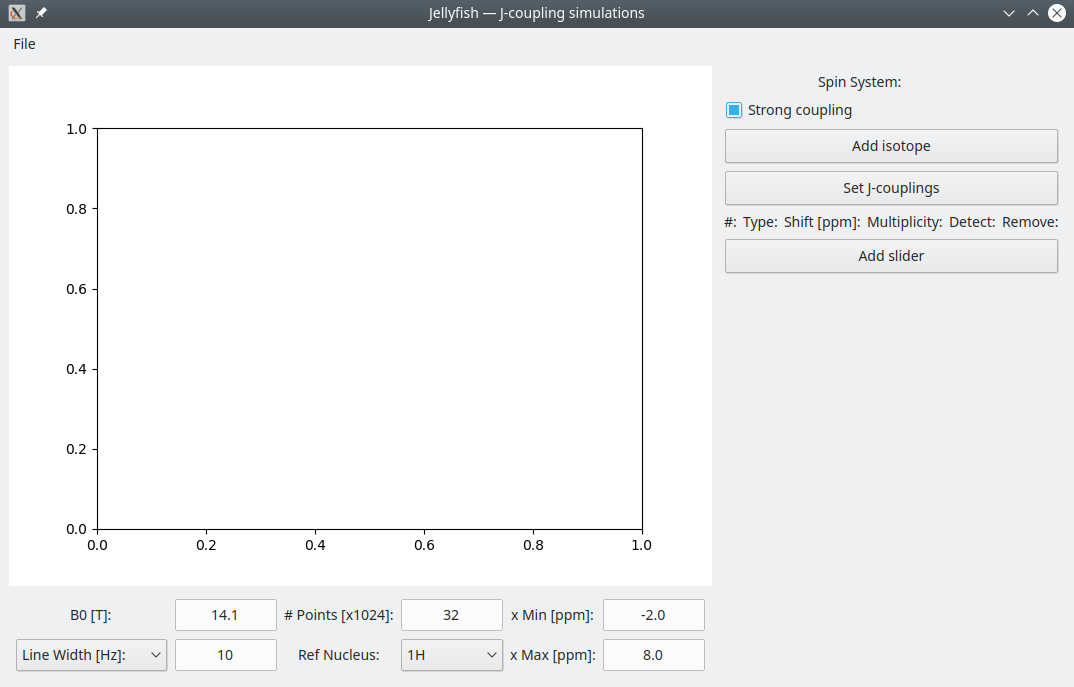
\includegraphics[width=0.8\linewidth]{Images/Interface1.png}
\end{center}

The window has two regions of settings: the spin system on the right, and the spectrum settings in
the bottom. Also, there is a plot region.

\subsection{Plot region}
There are several ways to control the display of the spectrum 
using the mouse. Below, a list of these is given:

\begin{itemize}
\item Dragging a box while holding the left mouse button creates a zoombox, 
  and will zoom to that region.
\item Dragging while holding the right mouse button drags (i.e.\ pans) the spectrum.
  Doing this while holding the Control button pans only the x-axis, holding Shift pans only the y-axis.
\item Double clicking with the right mouse button resets the view to fit the whole plot (both x and y).
\item Scrolling with the mouse wheel zooms the y-axis. Doing this while also holding the right mouse 
  button zooms the x-axis. By holding Control the zooming will use a larger step size.
\end{itemize}

\subsection{The bottom frame}
In the bottom frame, several parameters can be changed:
\begin{itemize}
  \item B0 [T]: the magnetic field strength in Tesla. This value can also be changed from a slider
	 (see below)
  \item Line Width [Hz/ppm]: the line broadening added to the spectrum simulation. Input either in
	 Hertz or ppm (can be changed via the dropdown menu). The ppm setting is most useful when
	 changing the magnetic field: the effective line width remains constant then.
  \item \# Points [x1014]: The number of points in the spectrum.
  \item Ref Nucleus: Defines the reference frequency (i.e.\ nucleus) of the spectrum.
  \item x Min [ppm]: The minimum x-value in ppm
  \item x Max [ppm]: The maximum x-value in ppm
\end{itemize}

\subsection{The spin system frame}
On the right-hand side of the window, the spin system can be defined. Jellyfish support spin
systems of any size (but your computer will not be able to handle very large systems, of course).
There are several buttons always available:
\begin{itemize}
  \item Strong coupling: toggle that determines if strong coupling is present. This determines if
	 the $J_{xy}$ part of the Hamiltonian is added. In realty, this is always on. The toggle is
	 provide here to be able to show the effect of this strong coupling.
  \item Add isotope: Adds an isotope to the spin system. The gives a pup-up window were the type of
	 nucleus can be selected, the chemical shift can be given, and the multiplicity defined. Pushing
	 OK adds this spin to the system. This adds a row of input boxes to the interface, were the shift
	 and multiplicity can be changed.
  \item Set J-couplings: Opens a window to set the J-coupling parameters. By default, all are 0. The
	 amount of entries depends on the spin-system that has been defined at the moment.
  \item Add slider: Adds a slider to the interface. This can be used to change a specific parameter
	 while watching the resulting spectrum. Ideal for teaching purposes on the effect of strong
	 coupling, field strengths, etc. Pushing this button opens an input window, where the type (B0,
	 Shift, or J-coupling) needs to be defined, as well as the minimum and maximum value of the
	 slider. For the `Shift' or `J-coupling' type, one or two spin numbers also need to be given.
\end{itemize}

When a spin is defined, an extra line is added to the interface with the following options:

\begin{itemize}
  \item Shift [ppm]: the chemical shift in ppm
  \item Multiplicity: the multiplicity of the nucleus (i.e.\ the $^1$H multiplicity of a CH$_3$ group is
	 `3')
  \item Detect: whether or not this nucleus is detected (i.e.\ added to the spectrum)
  \item X: remove this nucleus from the spin system. This also clears all relevant J-couplings, and
	 removes and slider that has a relation to this spin.
\end{itemize}
  
When a slider is defined, it adds a row to the slider space. Here, there now is a slider which can
be used to change the specified parameter. There is also a `X' button to remove the slider. When
using a slider, the respective value is also changed in the rest of the interface (e.g.\ chemical
shift are also updated in the spin system rows).


\subsection{Menu}
Jellyfish also has a menu on the top of the interface. It has the following options:

\begin{itemize}
  \item File:
\begin{itemize}
  \item Export Figure: export the current plot as an .png image.
  \item Export Data (ASCII): save the current spectrum as a text file (x and y data).
  \item Export as ssNake .mat: save spectrum as a Matlab file as used by the ssNake software (see
	 \url{https://www.ru.nl/science/magneticresonance/software/ssnake/}).
  \item Export as Simpson: save as a text file as supported by the Simpson simulation software
	 (see \url{http://inano.au.dk/about/research-centers/nmr/software/simpson/}).
  \item Quit: closes the program
\end{itemize}
\end{itemize}

\section{Running as a script}
Apart from running Jellyfish as a program via the user interface, it can also be used as a library
from within python. This requires that you have the source code of Jellyfish (and not a compiled
version). The `Examples' directory holds some examples on how to do simulations from a script. Below
an easy example is given. Here, it is assumed that the Jellyfish main directory (which holds
\texttt{engine.py}) is one directory higher than this file.

\lstset{language=python} 
\begin{lstlisting}[frame=single]  
import numpy as np
import sys
sys.path.append("..")
import engine as en

#-------Spectrum settings------------
Base = 42.577469e6
RefFreq = 600e6 #zero frequency
B0 = RefFreq/Base #B0 is proton freq divided by the base scale
StrongCoupling = True #Strong coupling on
Lb = 0.2 #Linewidth in Hz
NumPoints = 1024*128 #Number of points
Limits = np.array([-1,3]) #Limits of the plot in ppm

#-------Spin system------------
# add spin as ['Type',shift, multiplicity,Detect]
SpinList = [['1H',0,1,True]] 
SpinList.append(['1H',2,1,True])

Jmatrix = np.array([[0, 10],
                    [ 0, 0]])


#-------Make spectrum----------
# Prepare spinsys:
spinSysList = en.expandSpinsys(SpinList,Jmatrix) 
# Get frequencies and intensities
Freq, Int = en.getFreqInt(spinSysList, B0, StrongCoupling) 
# Make spectrum
Spectrum, Axis, RefFreq = en.MakeSpectrum(Int, Freq, 
					Limits, RefFreq,Lb,NumPoints) 
#Save as ssNake Matlab file
en.saveMatlabFile(Spectrum,Limits,RefFreq,Axis,'easy.mat')
\end{lstlisting}

\section{Technical background}
In the following, I will discussed the algorithms that are implemented in Jellyfish for
the simulation of strong coupling patterns. This part is both a documentation, as well as
a tutorial on how to approach these calculations. Any suggestions to improve the algorithm
are appreciated.

\subsection{Basics}
In order to simulate a spectrum, we need to know which frequencies are present, and the
amplitude of these frequencies. Based on that, we can draw a spectrum directly (as a
histogram), or simulate the FID (as a series of complex exponentials). Calculating the
spectrum directly is much faster, and this is used in Jellyfish. This is accurate if the
number of points is high enough.

In order to calculate the energies, we need the Hamiltonian of the system. The total
Hamiltonian is the Hamiltonian of all spins, including the Zeeman interaction (with the
chemical shift) and the scalar coupling (J-coupling) interaction between all pairs of
spins:
\begin{equation}
  \mathcal{H} = \sum_{i}{\mathcal{H}_{i}^\text{zee}} + \sum_{i}\sum_{s>i}{\mathcal{H}_{i,s}^\text{J}}
\end{equation}
Here, the double sum is only needed for a part of all pairs ([i,s] and [s,i] are equal,
and [i,i] = 0).

To get the energies of the transitions, we need to transform the Hamiltonian to a diagonal
frame (i.e.\ gets its eigenvalues)\footnote{Note that I
use the $\bullet$ symbol to represent a matrix multiplication, and a $\cdot$ for a
point-wise multiplication.}:
\begin{equation}
  \mathcal{H}^\text{int} = T^{-1} \bullet \mathcal{H}\bullet T
\end{equation}
where the `int' superscript indicates we have gone to the interaction frame.  Here $T$
represents the eigenfunction matrix, we we can use to transform the Hamiltonian to a new
frame. $T^{-1}$ is the inverse of this matrix. In this representation, the energy of
transition $i \rightarrow j$ is equal to $\mathcal{H}^\text{int}[i,i] -
\mathcal{H}^\text{int}[j,j]$.

Apart from the energy, we also need the transition probability, i.e.\ the intensity of the
transient. This depends on two things: the start operator, and the detection operator. We
use the following definitions\footnote{Note that I use $I_x$ to mean the Pauli matrix of
  the $\hat{I}_x$ operator. I will do this throughout this manual. All operators are in
their matrix form.}:
\begin{equation}
  \rho_0 = I_x
\end{equation}
as a starting operator. And
\begin{equation}
  \text{Detect} = I_+
\end{equation}
To get the probability of a transition, we multiply these values in a point-wise fashion:
$\rho_0 \cdot \text{Detect} = I_x  \cdot I_+$. However, we want this result to be defined
in the interaction frame:
\begin{equation}
  P = (T^{-1} \bullet I_x \bullet T) \cdot (T^{-1} \bullet I_+\bullet T)
\end{equation}
Having calculated this, we can get the intensity of transition $i \rightarrow j$ as $P[i,j]$.

\subsection{Hamiltonians}
The Zeeman Hamiltonian is (including Chemical shift effects):
\begin{equation}
  \mathcal{H}_\text{zee} = \sum_i B_0  \gamma_i (1 + \delta_i) I_z^i
\end{equation}
with $B_0$ the magnetic field strength in Tesla, $\gamma$ to gyromagnetic ratio of the
nucleus of interest in Hz/T and $\delta$ the chemical shift.

The scalar coupling Hamiltonian (J-coupling) is:
\begin{equation}
  \mathcal{H}^\text{J} = \sum_{i}\sum_{s>i}{\mathcal{H}_{i,s}^\text{J}} = 
  \sum_{i}\sum_{s>i}{J_{i,s}(I_x^i I_x^s + I_y^i I_y^s + I_z^i I_z^s)}
\end{equation}
with $J_{i,s}$ the scalar coupling value between nucleus $i$ and spin $s$.

Often, this Hamiltonian is split in apart that commutes with the Zeeman term (i.e.\ the
weak coupling part) and a part that does not commute: the strong coupling:

\begin{equation}
  \mathcal{H}^\text{J} = \mathcal{H}^\text{J}_\text{weak} +
  \mathcal{H}^\text{J}_\text{strong}
\end{equation}
with:
\begin{equation}
  \mathcal{H}^\text{J}_\text{weak} = \sum_{i}\sum_{s>i}{J_{i,s}(I_z^i I_z^j)}
\end{equation}
 and
\begin{equation}
  \mathcal{H}^\text{J}_\text{strong} = \sum_{i}\sum_{s>i}{J_{i,s}(I_x^i I_x^s + I_y^i
I_y^s)}
  \quad.
\end{equation}

Jellyfish makes use of the fact that the full Hamiltonian is always Hermitian: the lower
diagonals are the complex conjugate of the upper diagonals. Therefore, we construct a
matrix with only the upper diagonals, which still leads to the correct eigenfunctions an
eigenvalues using the \texttt{numpy} \texttt{eigh} routine. To demonstrate why this is of
use, I will describe some equalities using the \texttt{triu} function. This function returns
the matrix with only the diagonal, and upper diagonals retained.

We can rewrite the equation for the strong J-coupling in a more convenient way:
\begin{equation}
  \mathcal{H}^\text{J}_\text{strong} = \sum_{i}\sum_{s>i}{J_{i,s}(I_+^i I_-^s + I_-^i
I_+^s)/2}
\end{equation}
We can then write:
\begin{align}
\text{triu}(\mathcal{H}^\text{J}_\text{strong}) =& \sum_{i}\sum_{s>i}{J_{i,s}(\text{triu}(I_+
^i I_-^s) + \text{triu}(I_-^i I_+^s))/2} \\
=& \sum_{i}\sum_{s>i}{J_{i,s}(I_+^i I_-^s )/2}
\end{align}
Here, we use the fact that $I_+^iI_-^S$ only has non-zero values on the upper diagonals,
and $I_-^iI_+^S$ has no non-zero values on the upper diagonals. Naturally, this is faster
to calculate than the full Hamiltonian.


\subsection{Operator definitions}
To set up the Hamiltonian, as well as the start and detect operator, we need several one
and two spin operators to be defined. Above, I used $I$ to represent a spin operator. Note
that, in the Hamiltonians described above, $I$ must stand for the spin operator defined in
the full basis (i.e.\ taking all the spins into account). Below, I shall use $\mathfrak{I}$
to represent a spin operator in its own basis. 

In order to calculate, say, the $I_z^1$ operator (i.e.\ the $z$-operator of spin 1 in the
full basis), we take the operator in its own basis ($\mathfrak{I}_z^1$) and use the
Kronecker product ($\otimes$) to come to the full basis. For a 3 spin system:

\begin{equation}
  I_z^1 = \mathfrak{I}_z^1  \otimes \mathbb{1}^2 \otimes \mathbb{1}^3
\end{equation}
Here, $\mathbb{1}^i$ represents the identity matrix of spin $i$. The Kronecker product
works like:
\begin{align}
  \mathfrak{I}_z^1  \otimes \mathbb{1}^2 =&
  \begin{bmatrix}
	 -1/2 & 0 \\
	 0 & 1/2 \\
  \end{bmatrix}\otimes
 \begin{bmatrix}
	 1 & 0 \\
	 0 & 1 \\
  \end{bmatrix} = 
 \begin{bmatrix}
	 -1/2\begin{bmatrix}
	 1 & 0 \\
	 0 & 1 \\
  \end{bmatrix}	 
	 & 0 \begin{bmatrix}
	 1 & 0 \\
	 0 & 1 \\
  \end{bmatrix}\\
	 0 \begin{bmatrix}
	 1 & 0 \\
	 0 & 1 \\
  \end{bmatrix}& 1/2 \begin{bmatrix}
	 1 & 0 \\
	 0 & 1 \\
  \end{bmatrix}\\
  \end{bmatrix}\\
  =& \begin{bmatrix}
	 -1/2 & 0 & 0 & 0 \\
	 0 & -1/2 & 0 & 0\\
	 0 & 0 & 1/2 & 0\\
	 0 & 0 & 0 & 1/2\\
  \end{bmatrix}
\end{align}
for two spin 1/2 nuclei. Note here that this calculation is quite inefficient: a lot of
zeroes are calculated. Actually, for an $I_z$ operator in matrix form, we know beforehand
that we can expect only non-zero values along the diagonal.

In all cases, we only need the upper diagonal definitions of the operators. This is
because we use the Hermitian property of the Hamiltonian, and we need only the upper
diagonal transition probabilities. This means that we can use:
\begin{equation}
  \text{triu}(I_x) = I_+/2
  \label{eq:IxIp}
\end{equation}
which means we only need $I_+$ (and not $I_y$, $I_x$ or $I_-$). This is because $I_-$
is the complex transpose of $I_+$, and is therefore easily related to it.

The ideas described above lead to the fact the we need to know $Iz$ and $I_+$ for each
spin. We should establish these as efficient as possible. For both of these, we can
generate them as 1D arrays in first instance: both operators have only a single `order'
diagonal populated. For $I_z$ Jellyfish uses a 1D Kronecker product operation.


\subsection{Detection}
For the detection we need both $I_x$ (the start operator) and $I_+$ (the detection
operator). Using \autoref{eq:IxIp}, we can write this more efficiently:
\begin{equation}
  \text{triu}(P) = (T^{-1} \bullet \sum_i I_x^i \bullet T) \cdot (T^{-1} \bullet \sum_i I_+^i\bullet T)
  = 1/2 (T^{-1} \bullet \sum_i I_+^i\bullet T)\cdot (T^{-1} \bullet \sum_i I_+^i\bullet T) \quad .
\end{equation}
In this way, the two parts are equal, and only need to be calculated once.
Note that this is only valid if \textit{all} spins are detected. In the case were we do
not detect some spins, these should not be included in the $I_+$ part (the detection
operator) but must be include in the $I_x$ part. This makes the sums unequal.


\subsection{Speeding up: block diagonals}
One efficient way to speed up the calculation of the spectrum is to separate the total
matrix representation of the system into different blocks. We can do this if there are
eigenfunctions who have no matrix elements between them (i.e.\ no off-diagonal element).
These off-diagonal terms are cause by the strong J-coupling elements. The challenge is to
find these blocks in an efficient way.

The first trick we can use is called `total spin factorization'. In here, we separate the
Hamiltonian in parts which have equal total spin quantum number. This is based on the fact
that our J-Hamiltonian has $I_+^iI_-^S$ as a term. In order for there to be a non-zero
value between two states, the spin quantum number of spin $s$ should be able to lower 1,
and of spin $i$ to be raised one. This leads to a new state with the same total spin
quantum number! Therefore, two states that have a different total spin quantum number can
never be related, and can be treated as separate groups, i.e.\ as blocks within the
Hamiltonian.

The above is true in all cases. However, we know that if there are no J-couplings present,
$all$ states are blocks of there own. This means that there may be smaller blocks
depending on the actual problem. In order to find them, we make a list of all connections
between states. We then find all independent groups via the breadth first search (an
algorithm from graph theory). This takes time, but is often worth it in the end.

All found blocks are diagonalised on their own. In the detection, the eigenvectors of two
blocks are needed to find the intensities of the transitions between them (the detection
operator \textit{does} have terms between these groups!). This transformations via the $T$
terms are also quicker in this way, then for the full Hamiltonian.

\subsection{Speeding up: Composite Particle Model}
Another way to speed up calculations concerns the case where we have multiple identical
spins. In Jellyfish, this is input using the `multiplicity' option. Multiple spins are
identical if they have the same spin quantum number, chemical shift, and identical
couplings (if any) to all other spins. A clear case where this is true is for the $^1$H
nuclei in a CH$_3$ group.

Normally, we would treat this group as a system with $2^3 = 8$ energy levels. However, we
know that there can be no off-diagonal (J-terms) between these. Looking at this system in
more detail, we see that there are four energies, with intensities [1,3,3,1]. The trick
that we can use, is to spilt this system in multiple individual parts. This called the
Composite Particle Model (CPM). In this particular case, we can split this system of three
spin 1/2 nuclei into one spin 3/2 nucleus (intensities [1,1,1,1]) en two spin 1/2 nuclei
(intensity [0,2,2,0]). This gives us a size 4 and size 2 problem, instead of a single
size 8 problem. This is much faster, especially if the rest of the spin system is quite
large. Note that the two spin 1/2 subsystems are identical, so we calculate its spectrum
only once, and multiply by 2.

The method described above is valid for any group of identical nuclei. The intensities
follow exactly the same pattern this group of spins cause as a J-coupling effect on other
spins. For the example above, the three $^1$H spins cause a quartet ([1,3,3,1]). For four
spins, a quintet would ensue ([1,4,6,4,1]) which can be described as a spin 2 system,
three times a spin 1 system, and two times a spin 0 system.

Additional speedup can be achieved using the CPM by using symmetries. We use CPM to split
all the identical parts of the full spin system. We then have a whole set of individual
subsystems that we need to do the spectrum calculation on. Before we do that, we can
check if there are copies due to symmetry effects. Doing this doe snot require a user
input for the symmetry, but can just be check for all cases (naturally, user input to
supply the symmetry will also work, but Jellyfish is written to be generally applicable).



\section{Contact}
To contact the \texttt{Jellyfish} team write to \texttt{ssnake@science.ru.nl}.
%\bibliographystyle{BibStyle}
%\bibliography{ReferenceManual}

\end{document}
